\chapter{Introduction}

Creative open-ended evolution in artificial systems \parencite{Taylor2001} is motivated by the gap observed between the products of biological evolution, and those produced by artificial evolutionary systems. The goal is to address two shortcomings of current systems: first, the products of artificial evolution are missing “impressiveness” or the capacity to surprise; the most common reaction is that they lack creativity.\footnote{A creative system is one that produces artefacts that are novel, surprising and valuable (Boden 2004); properties that are desirable not only in the “creative” fields of art, literature, music and the like, but also in more prosaic areas such as engineering and indeed artificial evolutionary systems.} Second, artificial evolution today lacks “open-endedness”, or the capacity to continue to produce new variants. 

In this work, we examine one aspect of the emergence of open-ended evolution from low-level elements--a step in the transition from undifferentiated entities to entities constructed from inherited rules or information. 

The central element of the problem is well known (\eg, \textcite{Maynard-Smith:1995lw, Szathmary2000}): for open-ended evolution (evolution which can continue without exhausting its capacity for variation), the potential for variation must be very high: indeed the system must be capable of representing a larger number of types than there are entities \parencite{Szathmary1999}. In biological evolutionary theory, this type of replicator is sometimes known as a modular replicator (\eg \cite{Szathmary2000}) or more recently, an informational replicator (\textcite{Orgel1992} for an earlier sense, or \cite{Zachar2010}). 

The informational replicator terminology might be biological, but the concept is just as valid in artificial evolutionary systems--the common problem is one of stable informational storage. 

Unfortunately, the emergence of an informational replicator from low-level elements has been extremely hard to achieve in artificial systems, and remains an open problem. Previous work has either introduced handbuilt replicators (\eg \cite{Hutton2003}), or relied upon specific, non-evolvable scaffolding in the base system (\eg the h-copy operator in Avida \parencite{Ofria2004}.) No generic approach is known in the literature.

However, there is another, simpler, form of biological replicator that also can maintain information--the variable \parencite{Zachar2010}, or holistic replicator, of which composomes (compositional replicators \parencite{Segre1998}) are perhaps the best-known example. 

Although the gap from variable replicators to informational replicators seems large and the pathway from one to the other poorly understood, variable replicators have the great advantage that emergent examples seem feasible in low-level reaction systems. Existing work has modeled forms of variable replicator (\eg \cite{Vasas2012}) without showing their emergence--in this work we demonstrate this in a molecular \gls{achem}.

Furthermore, although variable replicators have well-established limitations as to the quantity of information that can be stored, we observe that previous work has generally modeled their behaviour in stable environments. Variable or changing environments have known effects on variation and range in macro-evolutionary systems, and we conjecture that this effect might well also apply at macro-molecular scales, so increasing the information storage capacity of a variable replicator.

\section{Motivation and context}

Biological evolution has produced ecosystems of astonishing variety and range, occupying essentially every viable niche on, above, and within the Earth from a common origin in the prebiotic world many millions of years ago. This has been far more than a working out of a single theme; instead a hugely impressive radiation of form and function has left that original ancestor far behind. The only connection that remains is the unbroken lineage of genes that links that earliest ancestor to every descendent organism alive today.

The origin of life was almost certainly contingent, and there is an absence of evidence from early stages \parencite{Pross2013}. There are many possible pathways, and unless some record remains somewhere (either geological or phylogenetic), the actual path is essentially lost to history.

However, a consensus is forming that early life began with chemoautotrophs fuelled by energy from inorganic redox couples and biomass from CO\textsubscript{2}, and that innovations in carbon-fixation created the main branches in the tree-of-life \parencite{Braakman2012}. 

The initiation of selection is marked by the advent of the \gls{ida}, probably from an RNA world, followed substantially later by the so-called \gls{luca} \parencite{Yarus2011}. It is important to note for clarity that \gls{luca} was almost certainly not a single entity or even species, but rather is a construct of evolutionary genetics because of the likely predominance of Lateral Gene Transfer (LGT) in archaic biology\footnote{http://sandwalk.blogspot.ca/2007/03/web-of-life.html}. 

Lateral or Horizontal Gene Transfer is thought to have been so common in early life that there was no single common ancestor, but rather genes from multiple lineages intermixed during this early stage into all lineages today \parencite{Ragan2009}. Although the advantages of a distinction between genome and phenome are discussed by many, including \parencite[section 7.2.3]{Taylor1999} and indirectly \textcite{VonNeumann1966}; there is no inherent dependency on this in \gls{ens}. Early evolution may have involved the inheritance of complete portions, or components, of the phenome before the advent of a distinct genome, while research into \gls{hgt} (\eg \textcite{Ochman2000,Pace:2008vi,Ragan2009}) has shown that not only was component transfer between species a major driver of early evolution, but a horizontal component-based mechanism continues to exist even in many of today's organisms that have a genome built from DNA. 

Two alternative models exist for the step from the prebiotic world  to \gls{ida} (\cref{major-stages-early-life}): replication- or genes- or RNA-first, and metabolism- or protein-first. Both metabolism and replication were almost certainly required for \gls{ida}, however. Self-replicating RNA enzymes are described in \textcite{Lincoln2009}, forming the basis of a selective system (also see \textcite{Cheng2010,Powner2009} for formation of RNA in prebiotic conditions). 

Some elements of \gls{ida}  are thought to still be with us in lineages of informational (for protein synthesis and RNA transcription) and operational genes (for some standard cellular processes) \parencite{Ragan2009}, for example the ribosome and ribonuclease P (RNase P) \parencite{Wilson2009}. The next major transition was to the Protein world, although predominance of RNA transcripts leads to suggestions that it should more accurately be called the RNA-Protein world \parencite{Altman2013}. 

A self-sustaining autocatalytic network (perhaps in the form of a \gls{raf} set, a ``set of molecules and reactions which is collectively autocatalytic in the sense that all molecules help in producing each other (through mutual catalysis, and supported by a food set)'' \parencite{Hordijk2011}) is generally considered essential \parencite{Pross2013}, but not sufficient \parencite{Hordijk2011}. Both competing models--replication-first and metabolism-first--build on this. In the case of replication-first, through autocatalysis as expressed by self-replication of oligomeric compounds; in metabolism-first, by cycles and networks. From another perspective, metabolism-first privileges function, while replication-first privileges descent.

The main difficulty with the replication-first model concerns the sizeable step required from abiotic compounds to template-based, or information-based, replication (although ribonucleotides conceivably could form in pre-life conditions \parencite{Powner2009}). Templates encode information in biology, so template-based replication requires an encode/decode mechanism as well as an information code. This is significantly more complex than simple duplication. By contrast, the main issue with the metabolism-first model concerns the necessary shift from composomal or holistic\footnote{See discussion in \cref{variable-replicators}.} inheritance to template-based, and the ability of holistic systems to represent a sufficient range of stable states for unrestricted evolution \parencite{Vasas2010}.

The origin of life can be seen as the transition from chemistry to biology, and seems tantalizingly close to the artificial evolutionary goal of moving from simple, uninteresting, systems to creative systems which evolve. However, the usefulness of the similarity is limited: the primary postulates of origins of life research are not our postulates. Most abiogenesis resarch assumes real-world chemistry and conditions, a constraint that doesn't apply to \gls{alife} or artificial \gls{oe}, and so is far more restrictive than required. 

\begin{figure}
	\begin{center}
		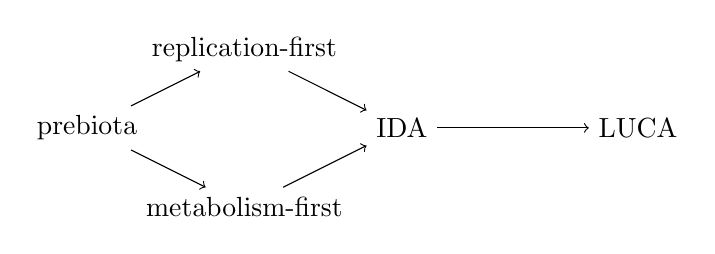
\begin{tikzpicture}
		\node (prebiota) at (0,0) {prebiota};
		\node (metabolism-first) at (2,-1) {metabolism-first} edge [<-] (prebiota);
		\node (replication-first) at (2,1) {replication-first} edge [<-] (prebiota);
		\node (ida) at (4,0) {IDA} edge [<-] (replication-first) edge [<-] (metabolism-first);
		\node (luca) at (7,0) {LUCA} edge [<-] (ida);
		\end{tikzpicture}
	\end{center}
	\caption{Some of the stages proposed in the evolution of early life}
	\label{major-stages-early-life}
\end{figure}

\section{Previous work}\label{previous-work}

Heredity is one of the foundational elements of \gls{ens}, the means by which information from one generation can be leveraged in the next. This form of inheritance, from parent to child, is called \emph{vertical} inheritance, and the type of entity that participates in and enables vertical inheritance (that is, can form a child) is called a \emph{replicator}. 

In the transfer from the prebiotic world to the biotic one, the proportion of information held by a predecessor that could be passed on to its successor increased, over many generations, from ``none'' to ``nearly all''. \Textcite{Vasas2012a} relate heritability to the correlation between the parent and child entities. Heredity is therefore likely a matter of degree, rather than being a binary relationship (related or not-related), and that opens up the possibility that a series of gradual changes might over time transform a very poor replicator into a very good one. Of course, one possible process for this transformation might well be \gls{ens}.

This progression is comprehensively explored in \textcite{Zachar2010}, extending earlier work by \textcite{Szathmary1999,Szathmary:2006ty}: 

''The simplest of replicators is the \emph{exact replicator}, which is \emph{non-informational}, and any change made to it causes a change in the phenotype. If a variation can arise in the structure in such a way that it does not change equivalence of the entity, then it is a \emph{variable} replicator, with more than one stable state. If such changes can be passed on to the offspring then the replicator is \emph{informational}. If the non-heritable part is constructed by a developmental process, then the replicator is a \emph{reproducer}.'' \parencite[p.21]{Zachar2010}\footnote{Interestingly, in biology at least, the starting point for the development of modern replicators might have began with \emph{horizontal} inheritance. By analogy, it’s easy to envisage another kind of information transfer where information is passed from one entity to another horizontally, without replication or a parent-child relationship. In today’s biology, \gls{hgt} provides one mechanism for this; in the early prebiotic world, the horizontal transfer of information might have occurred through a number of conceptually similar mechanisms (such as auto-catalytic cores) that didn’t involve genes. 

First, the changes from horizontal inheritance can be heritable in a vertical sense. In organisms with genes, by definition under \gls{hgt} the change becomes part of the target’s genome and hence heritable. In entities without genes, there are forms of entity where the horizontal change can be subsequently inherited vertically. Second, mechanisms for horizontal transfer don’t require replication (by definition). Therefore it’s possible that they can act as a precursor for the development of replication. That is, horizontal inheritance plus selection might be sufficient for replication, rather than replication being required for inheritance.}

But what exactly does it mean for something to be a replicator? Is a rock that erodes to form grains of sand a replicator\footnote{In \textcite{Bourrat2015} rocks are given as examples of \emph{persistors}, unable to reproduce and subject to only a ``weak'' form of selection for hardness}? Is a set of autocatalytic reactions that splits into two replicating? \Textcite{Dawkins1976} was the first to define replicators, including a range from biological genes to non-biological ideas (memes) in the scope of the definition. Many other definitions and formulations followed as various properties or features were examined. 

%\textcite{Hogeweg1998} describes attractor-based heredity (inheritance of state) and storage-based. 
%
%Heredity by \textcite{MaynardSmith1999} is modular or holistic--if module changed only that module changes in descendants, holistic change part changes whole. Believe it true that unlimited heredity implies modular. \textcite{Szathmary1999} calls these digital and holistic, and adds phenotypic replicators whereby ``phenotype or function of one object is translated to the other, without any modular copying effect” 
%
%Modular/template heredity has advantages of: mutations hereditary; problems of correct copying \parencite{Eigen1977}

Relatively recently, \textcite{Zachar2010} saw a need to reexamine the definition primarily to resolve issues of discrimination between entities which are clearly replicators or not replicators and those which are borderline, and between biological replicators and non-biological or cultural ones. 

%A regenerating/recreating entity can produce at least one entity equivalent to it. It is possible that the original entity immediately decomposes (that is, cannot be the subject of further turns of the cycle), causing sequential replacement, although this is the most simple of regenerating entities. If it can effectively increase the number of entities equivalent to itself, then it is autocatalytic and is a \emph{replicator}.

\Textcite{Zachar2010} conclude that a replicator is ``any autocatalytic entity for which there is a selection process defined'', using autocatalysis in the general sense of a cyclical process that increases $A$ by $\Sigma x_i + A\rightarrow \Sigma y_j + \Sigma B_k$ (where $n$ of the ${B_0, B_1...B_k}$ products are equivalent to $A$), and where selection has the fairly standard definition of ``a process, acting on a particular population of entities in a particular environment, which sorts entities according to their phenotypes.'' \parencite[p.21]{Zachar2010}

In the following \namecrefs{non-informational-exact-replicators} we review some pertinent previous work following the classification developed in \textcite{Zachar2010}\footnote{With the exception of \emph{reproducers} (replicators with a developmental component) as these extend informational replicators.}.

\subsection{Exact replicators}\label{non-informational-exact-replicators}

Autocatalysis by definition is replication; if the entities are molecules, the autocatalytic reaction $\Sigma x_i + A\rightarrow \Sigma y_j + \Sigma B_k$ replicates the molecule $A$ (\eg \textcite{Lifson1997}). Evolutionary variation though is difficult as the exponential growth of the main autocatalytic product will generally overwhelm the molecules produced by any side reactions unless 1) they are also autocatalytic, and 2) the solution contains the molecules needed to initiate and maintain this alternate autocatalysis cycle.

%GGL/ToyChem \textcite{Benko2003,Benko2005}                        	&Atoms/Molecules&&None--at level of reactions\\	
%RBN-World \textcite{Faulconbridge2011}                            	&Boolean Networks and Graphs& None--at level of ACS\\

\emph{RBN-World} \parencite{Faulconbridge2011} is a \gls{achem} where the entities take the form of \gls{rbn} \parencite{Kauffman:1969ne}, with the addition of a bonding mechanisms to allow for their composition and decomposition. The resulting form of \gls{rbn} is called a bonding \gls{rbn} or bRBN.  Larger structures are formed by ``bonding'' two independent bRBNs at each bRBNs bonding node. ``All reactions are between two reactants; it is assumed that more complicated reactions can be expressed as a series of two-reactant reactions with intermediate structures.'' The choice of reactants is described as ``Gillespie-like'', and essentially random, uncorrelated in any way with reaction energies or rates \parencite[chap.8]{Faulconbridge2011}.

Each bRBN is a synchronous RBN, made up of a number of nodes, each with an initial state (\emph{true} or \emph{false}) assigned randomly and with an input/output matrix assigned randomly. Finally k(=2) inputs are established per node. The bonding method uses ``cycle length as the bonding property and equality as the bonding criterion....bonds only exist between bRBNs that have the same cycle length.'' After initial bond formation the algorithm recalculates cycle lengths, and checks again for equality. This might result then in decomposition (records are kept of composition operations so that the reverse decomposition can be easily done.)

A number of parameters affect the behaviour of the chemistry, and so a series of experiments sampled from the parameter-space, and then used a GA, to search for interesting variants as measured by non-catalysed ``loops'' (as the preferred measures of auto-catalytic sets and \glspl{hypercycle} are too rare for use as a measure) \parencite[chap.8]{Faulconbridge2011}. 

The development of RBN-World involved many design choices, some essentially adhoc, such as the choice of \gls{rbn}: ``...the choice to use RBNs as the sub-symbolic representation in RBN-World was based on limited information. As a discrete dynamical system that is computationally tractable yet also spans a wide range of behaviours, RBNs met the appropriate criteria. It is not expected that RBNs are the best representation however; others may be more suitable for particular emergent properties.''

The model for \emph{Chemical Evolution by Natural Selection} in \textcite{Fernando:2008xy,Fernando:2007pf} is driven by origin-of-life objectives (``the evolution of chemical networks that lead to autonomous systems''), and takes the form of a simulation of laboratory experiments of lipid aggregates (``phase separated ‘individuals’, e.g. liposomes'') in a reactor. The molecules and food molecules (that make up an autocatalytic cycle) share a common representation and underlying chemistry, while replication, unlike the (rare) autocatalytic cycles in \textcite{Faulconbridge2011}, is by `` division by externally imposed agitation, i.e. replication rather than self-replication.''. New molecular species (evolutionary variation), comes from chemical ``avalanches'' initiated when two existing species are chosen at random, tested to see if a reaction between them is possible by thermodynamics, and then the resulting products seeded in the reactor at low concentrations. These new reactions may be autocatalytic, or the products may complete a food-set for another autocatalytic reaction, or they may enable a side-reaction from an existing autocatalytic one. Introducing these new species into the reactor therefore can trigger the rapid formation of a series of novel products--a chemical avalanche.

\subsection{Variable replicators}\label{variable-replicators}

\Textcite{Ganti:2003hl} and  \textcite{Eigen1971} showed that distinct, organisationally different alternative autocatalytic networks in the same environment might compete, and the fittest would prevail. A number of models have been proposed since where autocatalytic networks form stable components that can be inherited in a modular fashion in a process called compositional inheritance. All these models are analytical in nature, in many cases based on the \gls{ode} model of \cite{Farmer1986}.

%\emph{Reflexively Autocatalytic Polymer Networks} (RAPN) \parencite{Kauffman1986} are evolvable. First, likelihood of such networks higher than expected (Hordijk and Steel) and second, in \textcite{Vasas2012} putting these networks into compartments (so not well-stirred) then can do directional selection.

In the most well-known of these models, the Graded Autocatalysis Replication Domain (\emph{GARD}) model \parencite{Segre1998}, highly catalytic molecules determine the properties of the compotype (compositional genotype), and these are not necessarily inherited equally. Instead a child may, or may not, inherit one of these molecules and so its properties may be similar to or very different from its parent \parencite{Vasas2015, Vasas2012, Vasas2012a}. Information fidelity varies widely; the Eigen threshold \parencite{Eigen1971} applies, and mutation rates overwhelm selection \parencite{Vasas2015, Vasas2012, Vasas2012a}.

Mutations in cycles \parencite{Vasas2012a} are generally not heritable as mutant copies are rarely functional in autocatalysis. This makes mutation problematic as a source of variation in these autocatalytic systems; one alternative to mutations is avalanches, to form new cycles from the side-products of the base networks (as discussed in the previous \namecref{non-informational-exact-replicators})

% Any molecule in the core will produce the remaining species in both the core and periphery \parencite{Vasas2012a} and so reconstitute the core,

The model of \cite{Vasas2015, Vasas2012, Vasas2012a}, derived from \cite{Farmer1986}, tests the GARD hypothesis that compositional inheritance is possible where there is a parent-offspring correlation in molecular composition. The mechanism is autocatalytic cores made up of one or more linked autocatalytic loops to provide the compotype. The core forms an attractor, where one core equals one attractor, but multiple cores are required of course for selection. Multiple cores (produced by inhibition \textcite{Vasas2012a}) provide multiple attractors, but the attractors must be stable for selection to be stable and meaningful. Unlike GARD, which generates only single-core networks, the model in Vasas is capable of multiple cores, but as cores are the equivalent of a single bit of heritable information, it's hard to see core-based inheritance being capable of unrestricted heredity--there are practical limits to the number of stable cores that can co-exist in a system. 

\subsection{Informational replicators with shortcut replication mechanism}

A \emph{shortcut} is where the replication mechanism is directly implemented by the experimenter rather than being an emergent property \parencite{BanzhafBaumgaertnerBeslonEtAl2016}. As the mechanism is external to the entity it is not under selection; shortcut replicators are not, by our definition, open-ended. One of the most well-known systems with a shortcut replication system is Squirm3.

\emph{Squirm3} \parencite{Hutton2007,Hutton2002}. An artificial system capable of life-like \gls{oe} (creativity), initially developed with the goal of testing the hypothesis of \textcite{Taylor2001} \parencite[p.341]{Hutton2002}.

All elements in Squirm3 are constructed from atoms defined by \emph{types} (e.g., a, b, c\dots) and \emph{states} (e.g., 0, 1, 2\dots). Atoms and hence molecules are located on a 2D grid, and molecules cannot overlap or pass through each other. All reaction rules, such as \emph{R1: e8 + e0 $\rightarrow$ e4e3}, are pre-specified (\textcite[p.4]{Hutton2007} and \textcite[p.49]{Faulconbridge2011}), and a shortcut consisting of a set of eight rules in \textcite{Hutton2002} is sufficient to replicate single molecules. As all reaction rules, including those responsible for replication and hence inheritance, are exogenous to the model, the inheritance mechanism in Squirm3 is not evolvable. 

Individual entities in \textcite{Hutton2002} are simply single molecules. \Textcite{Hutton2007} introduces cells made up of a collection of molecules and bounded by a membrane of a particular atom type of limited reactivity; the membrane is intended to allow individuals to benefit from innovations by protecting their internal reactions from others. With a greatly increased set of predefined reaction rules (34 rules now for the cell replication shortcut, extended further again in \textcite{Lucht2012}), each cell has the capacity for division and mutation (through the stochastic application of equally applicable rules).  Selection is purely by indirect competition for the raw materials (atoms in the environment) required by the reactions in a cell; interactions between individuals are purely through this indirect competition (niche construction without direct interaction). Cells in \textcite{Hutton2007} are incapable of making use of resources from other cells (as they are effectively protected by non-reactant membranes) and so an intermittent exogenous mechanism (``floods'') is used to return the atoms in a number of randomly chosen cells to the environment.

There are however some difficulties in establishing anything more than a ``variable replicator'' (in the term of \textcite{Zachar2010}), namely inconsistent inheritance and a limited potential for information transmission. For this, we turn to informational replicators.

\subsection{Informational replicators or self-replicators}
Replication in these systems emerges from the base (or in the terminology of \textcite{BanzhafBaumgaertnerBeslonEtAl2016}, level-0) rules without being directly specified by the experimenter or designer. However, even here most systems still shortcut this by providing a seed or universal ancestor (\eg \textcite{Ofria2004}) that contains a working module for replication that can be then modified (for good or ill) in each subsequent generation.

\subsubsection{String-manipulation systems}

A new object in Fontana's Algorithmic Chemistry, or \emph{AlChemy} \parencite{Fontana1992}, is defined as the interaction expression, $h$, of two randomly chosen objects $f$ and $g$, if, and only if, the interaction expression contains at least one variable and one primitive operator, and is shorter than some maximum length \parencite[p.173--p.180]{Fontana1992}. New objects in AlChemy are therefore the children of two parents.

How then is the interaction expression $(('f)('g))$ between $f$ and $g$ evaluated to produce $h$? AlChemy is a form of pure LISP (with some ``minor idiosyncrasies''), based on toyLISP, with six primitive operators defined in \textcite[p.205]{Fontana1992}. The interaction expression is defined in \textcite[Definition A.9, p.204]{Fontana1992} as $V[(('f)('g)),()] = (V[f,(a\leftarrow g)])$, using the notation $V[e,L]=v$ to mean the expression $e$ with the ``association list'' $L$ (a list of value assignments between atoms and expressions) evaluates to $v$. The result $h$ is described as $f(g)$ and the process as $f+g \rightarrow (('f)('g)) \rightarrow h + f + g$.

Clearly reproduction in AlChemy is self-referential--the process to construct a child object is defined in the code of the parent objects. Unfortunately, inheritance doesn't follow straightforwardly as the reproduction process is unusual in two important ways. First, each new object has two parents, rather than one, as is more common in artificial systems (although not necessarily in biology.) Producing new objects as some function of the two parents in turn means that the relationship between parents and child is not a straightforward mutation or other syntactic difference, but rather a complex functional relationship. What this means for the relationship between the parent's fitness and the child's fitness is not obvious. It seems that the fitness differences in AlChemy might be more extreme than in other systems where parent and child have a more straightforward relationship.

%\begin{DRAFT}
%\parencite{Fenizio2000}:
%
%Original AlChemy reactions of form $A+B\rightarrow C$ where $C$ replaces an existing element.
%
%This system generates $A+B\rightarrow C_1+C_2...C_n$ where $C$ is a multiset of size $n$. Done by modifying the original K rule to detach x2 and eliminate both original elements (like reactants in chemistry)
%
%Uses combinators rather than lambdas
%
%To prevent from stopping (out of elements) added modification where randomly add/remove some elements
%
%Combinator first combines (appends) elements, each element other than first bracketed. Then each 1-term combinator applied to string, where it makes specific changes \eg K x1x2s0-\textgreater{}x1s0 (s0 is remaining substring, may be null). Apply until no further reductions possible (that is, in normal form). Two combinators are equivalent if can be reduced to same combinator (and previously noted that order is not important--same results regardless of order).
%
%Free pool of atoms for conservation of ``mass''
%
%\parencite{Fenizio2001}:
%
%Experiment to show spontaneous formation of autopoietic cells, with a focus on ``identity as an entity separated from its environment'', that is, membrane formation. Graph used to model spatial structures: ``an artificial chemistry (AC) is embedded in a graph, with each molecule being a vertex of the graph and possible interactions being allowed only along the edges of the graph''. Molecules are composed of atoms taken from a 
%
%``Molecules are built from a substrate of elements called atoms. There are seven types of atoms ($I, K, W, R, B, C, S$), each with a different function. The total number of atoms in the reactor is kept constant during a run. Free atoms (not bounded in molecules) are separately stored and form a global pool.''
%
%As the rules for the combinations of two molecules are predetermined (the reaction mechanisms are described in \textcite{Fenizio2000}), this model is not by our definition open-ended.
%\end{DRAFT}
\subsubsection{Automata}

\emph{Coreworld} \parencite{Rasmussen1990}, inspired by the early computer game ``Core War''\footnote{See \url{corewar.co.uk}}, set segments of simplified assembly code into competition in core memory. The assembly command to copy values from one memory location to another can spontaneously introduce errors into the copying, and hence can introduce evolutionary variation. However, as reviewed by \textcite{Ofria2004}, the system ``collapsed into a non-living state'' perhaps because organisms could copy over each other in the shared system memory \parencite{Ofria2004}.

In \emph{Tierra} \parencite{Ray1991} mutations are introduced during replication by randomly flipping bits during the copy operation (at a given rate of generally between 1 bit flip per 1,000 and 2,500 instructions copied). This rate is set by the experimenter, and is not evolvable. Mutations can also be introduced by the copy algorithm itself; as it is an algorithm defined in the organism in standard Tierra instructions (and hence fully embedded), mutations in the algorithm during a copy will be inherited by the child. The initial copy algorithm is part of the 80-instruction ancestral creature documented in \textcite[app.C]{Ray1991}.

In Ray's words, ``...this approach involves engineering over the early history of life to design complex evolvable organisms, and then attempting to create conditions that will set off a spontaneous evolutionary process of increasing diversity and complexity of organisms'' \parencite[p.3]{Ray1991}. As Taylor criticises though, the problem with ``engineering over'' is that we don't understand the natural examples well enough to engineer them at all \parencite{Taylor2001}

Tierra has been the testbed for a number of other works. For example, \textcite{SugiuraSuzukiShioseEtAl2003} converted Tierra into a string manipulation systems, introducing a set of 140 regular-expression based rewriting rules where each rule encoded one or more of the original 32 Tierran instructions. The initial rewriting ruleset was manually generated by the experimenters, although details are unclear. Unlike in Tierra where the instruction set is fixed during a run, the rewriting ruleset for each organism itself could evolve through a separate genetic algorithm. This algorithm removed the least applied rules and inserted the same number of new rules generated by mutating (through duplication, removal and addition of operations) a selection of the most applied rules. Although results support the claim that the ruleset as well as the genome evolves, the use of a separate genetic algorithm for ruleset evolution artificially separates the ruleset from the genome--the feedback loop from genome back to ruleset is broken.

Tierra was also the starting point for \textcite{Taylor2001, Taylor:1999sc} to explore the creation of \gls{alife}, by adding cell regulation, parallel processes and energy modelling \textcite[p.4]{Taylor:1999sc}.

% Seed (proto-DNA) must itself be an indefinite heredity replicator {[}assumes that this is minimal starting point, rather than that this itself may evolve{]} \parencite{Taylor2001}
%Assume that early stages see A+B implicitly encoded in the environment, essentially as simpler than explicit mechanism, but little justification given beyond ``At the early stages of an evolutionary process, however, we would not expect there to be mechanisms for explicitly decoding the proto-DNA\ldots{}'' \parencite{Taylor2001}

\emph{Avida} \parencite{Ofria2004}, introduced in the summer of 1993, based on Tierra with improvements including better metering and measuring, and a 2D lattice or well-stirred reaction vessel topography (unlike the shared linear memory of Tierra, for example). ``In principle, the only assumption made about these self-replicating automata in the core Avida software is that their initial state can be described by a string of symbols (their genome) and that they autonomously produce offspring organisms. However, in practice our work has focused on automata with a simple von Neumann architecture that operate on an assembly-like language inspired by the Tierra system.''

Like Tierra, the automata engine in Avida is based on a Turing tape-like metaphor, with instruction, read, write, and flow control heads that can be moved forward and backwards through memory using relative rather than absolute addressing. Instructions are grouped into instruction sets, with the default set containing 26 instructions, and by definition every program is valid. Each organism runs on its own virtual automata; the only interaction between organisms is via resources in the shared environment and through competition for virtual machine CPU cycles based on ``merit'' or fitness. Direct Tierra-style interactions by insertion of code into another organism is not enabled by default, but is possible through configuration. Phenotypes take the form of computations (entities take in resources, perform computations that result in merit, and perhaps produce output or by-product resources): ``\ldots by inputting numbers from the environment, performing computations on those numbers, and outputting the results. The organisms receive a benefit for performing specific computations associated with resources'' \parencite{Ofria2004}. Interestingly, the resources in the environment are not the same as the elements of the organisms (instructions from an instruction set.) Avidan organisms are not fully-embedded in their environment.

New organisms are created asexually by the parent first allocating memory for a child. The parent's read-head is placed at the beginning of its code, the write-head placed at the start of the newly allocated memory and successive h-copy instructions copy the instruction from the read-head to the write-head and advance both. Either once all instructions have been copied (or perhaps before) h-divide splits the child from the parent (all instructions between read-head and write-head go to the child) and starts both executing in a clean state. Variation is introduced through mutations which can be introduced through either h-copy (the write-head writes a random instruction rather than the instruction at the read-head) or in h-divide (a single random instruction may be deleted or added from the child code). Both forms of mutation happen with a fixed probability set by the inventor: COPY\_MUT\_PROB, INS\_MUT\_PROB, and DEL\_MUT\_PROB for h-copy, and DIVIDE\_INS\_PROB, DIVIDE\_DEL\_PROB for h-divide. However, there is a second, evolvable source of mutations during replication--the replication process itself is embedded in the organism, as a set of instructions, and so changes to this algorithm during the copy will persist in the child. The self-replication algorithm is initially defined in the ancestral organism used to seed a run, and as documented in \textcite[A1.3]{Ofria2004} consists of 15 instructions.

Avida is extremely configurable, but provides little guidance or theoretical justification for any particular configuration. Indeed this variability allows it to function most usefully as a general testbed for experiments, \eg ``in one experiment we wanted to study a population that could not adapt, but that would nevertheless accumulate deleterious or neutral mutations through drift'' \parencite{Ofria2004}.

\emph{Amoeba-II} \parencite{Pargellis2001} shares similar features to Tierra and Avida in that it is an instruction-set based automata, but unlike in those systems, replication spontaneously emerges in Amoeba-II. The replication process requires four steps: ``register initiation, memory allocation, copying of the parent's instructions to the child (embryo), and division where the child is initiated as a cell on its own'' \parencite[p.69]{Pargellis2001}. Two specific instructions in the parent's genome are required at a minimum. The MALL command allocates memory, and a virtual CPU to the child, and DIVD performs the division. Register initiation and copying of the parent's instructions can be done in a variety of different ways, and a good deal of the interest of the Amoeba-II system lies in the evolvability of these mechanisms. Selection is by efficiency of replication, where faster and more efficient replicators replace less efficient ones in the population (as \textcite{Pargellis2001} says, ``Amoeba has only one task: replication'') and so there is selective pressure from the least efficient, but functioning, mechanisms in the direction of improved replication. To complement selection and inheritance, variability is provided by the DIVD instruction, which introduces a mix of instruction substitutions, deletions and insertions into the child's program at a fixed but low rate.

Inheritance in Amoeba-II is almost too effective. Fit organisms rapidly evolve into extremely rapid reproducers and out-replicate all other entities, leaving a mono-culture \parencite{Pargellis2001}.

%\begin{DRAFT}
%\textcite{Dittrich1998}:
%A simulation approach towards ``dynamic phenomena, especially on the emergence of prebiotic evolution'', based on an artificial chemistry.
%
%Introduction of \textless{}\emph{S},\emph{R},\emph{A}\textgreater{} classification scheme for artificial chemistry, elaborated in \parencite{Dittrich:2001zr}, where in this work \emph{S} are `` binary strings with a constant length of 32 bits'', \emph{R} are of the form $s1+s2 \rightarrow s3$, and \emph{A} ''simulates a well-stirred tank reactor with mass-action kinetics, which assures that the probability of a collision is proportional to the product of the concentration of the colliding objects'' (based on earlier work by Fontana and Kauffman.)
%
%A=``1. Select two objects s1,s2 from the soup randomly, without removing them. 2. If there exists a reaction s1 + s2 to s3 and the filter condition f (s1,s2,s3) holds, replace a randomly selected object of the soup by s3.'', s1 and s2 are not consumed, rather they act as catalysts. Chosen as this shown capable of hypercyclic organisation
%
%Asn automata reaction with a set of operations (six common logic operations, \eg OR, and nine computational instructions), represented as 4-bit sequences, to generate s3 from s1, s2. Automata is a deterministic FSA, running s1 on s2 to produce s3. As Dittrich observes ``The first noticeable property is that the structure of the product s3 is similar to its 'parents' s1; s2. This indicates that there is a correlation between s1, s2, and s3 that is a prerequisite for evolution.''
%
%Passive self-replicators ($s1 + s2 \rightarrow s2$) are relatively common (approx. 30\% of randomly generated strings), while active self-replicators ($s1 + s2 \rightarrow s1$) are very rare (around 0.004\%).
%\end{DRAFT}
\subsubsection{StringMol and GraphMol}

\emph{StringMol} \parencite{Hickinbotham2011} and the related \emph{GraphMol} \parencite{Nellis2012, Nellis2014} explore computational novelty through embodiment: ``Our aim is to improve novelty-generation algorithms by making their biological models richer.'' No measure is proposed for novelty--the author's state that they're not even sure it is possible, but an informal definition is used that sees novelty as the outcome of increasing embodiment \parencite[p.87]{Nellis2012}. 

The base elements in StringMol are single-character symbols, each representing a microcode instruction. These combine to form molecular microprograms (the strings of the name). The general arrangement feels very similar to that in Avida or Tierra, complete with a variety of points (instruction, read, write, and flow for iterations).

GraphMol instead is graph based. ``The world defined by GraphMol contains chemicals (represented as graphs) that bind to each other via multiple binding sites, and then run simple computer programs (encoded in the graphs) that modify the binding of these chemicals.''. No explicit rationale for graphs is presented, other than as a natural extension from StringMol given the stated importance of a rich binding mechanism. 

An underlying principle in both systems is that the mechanism of evolution must be itself evolvable; functions such as template copying must be embodied mechanisms in the world so that they can be affected by evolution, and so evolved.  Crucially therefore both StringMol and GraphMol have embodied template copying, where a ``replicase'' molecule can copy another following the algorithm in \cref{alg:stringmolgraphmol}.

\begin{algorithm}[ht]
	$\text{i} \leftarrow \text{start(string B)}$\;
	\While{$\text{i not at-end(string B)}$}{
		$\text{string A(i)} \leftarrow \text{char-copy(string B(i)))}$\;
		$\text{i} \leftarrow \text{next i}$\;
	}
	\caption[The algorithm for template copying used by StringMol and GraphMol]{The algorithm for template copying used by StringMol and GraphMol, from \textcite{Nellis2014}}
	\label{alg:stringmolgraphmol}
\end{algorithm}

Each of the four functions in \cref{alg:stringmolgraphmol}--\emph{start}, \emph{at-end}, \emph{char-copy} and \emph{next}--can be either ``crisp'' (\ie perfect) or embodied (variable, and subject to evolution). As an example of an embodied function, StringMol's \emph{start} function uses pattern-matching to determine the binding region between the replicase and the other string where the replicase should begin copying. By changing the subsequences in either string the strength of bind can be varied, with a corresponding shift to the beginning of the copy region even though the pattern-matching algorithm itself does not change (it is a ``level-0'' component in the terminology of \textcite{BanzhafBaumgaertnerBeslonEtAl2016}). The same pattern-matching is used in StringMol's \emph{at-end} function to determine the end of the region to be copied.

StringMol includes an embodied \emph{start} and \emph{at-end}, crisp \emph{next}, and stochastic \emph{char-copy}; GraphMol has an embodied \emph{start}, \emph{at-end} and \emph{next}, with a crisp \emph{char-copy}. The primary difference between the two is opposite approaches to \emph{next} (``in order to investigate a method of embodying the copying process that would be completely different from Stringmol's.'' \parencite[p.145]{Nellis2012})

These mechanism differences (the choices of which functions are crisp and which are embodied) result in different outcomes for the overall system: ``Stringmol exhibits macro-mutation and two chemical copying; GraphMol exhibits two types of quasispecies, cooperative and parasitic. These two systems use the same domain (emergent evolution) and metamodel (machines copying strings), but different computational models.'' Other combinations would presumably show different behaviour again.

Despite the use of the term ``embodied'', those functions that aren't ``crisp'' are not in fact fully self-referential as the pattern-matching algorithm itself remains unaffected by evolution. There is also a disconnect between the properties of the targets of the matches and the functioning of the algorithm. The algorithm matches on the symbol, and is completely unaffected by the meaning or properties of those symbols, the underlying microcode. In this it differs significantly from a completely endogenous system such as a biological replicase, where the match or bind is actioned by the same chemical rules that construct and maintain the replicase from component atoms.

\subsection{Discussion}

Of the forms of replicator examined here, only full informational replicators provide both the representational range and the evolutionary flexibility for open-ended evolution. 

Exact replicators lack heredity as they cannot pass on variability to their descendents; variable replicators are capable of only a limited number of distinct states and so suffer from a restricted representational range; informational replicators based on shortcuts are evolutionarily restricted in that their inheritance/heredity mechanism is not evolvable. 

The systems reviewed in this \namecref{previous-work} follow different approaches, but none reach the goal of informational replication. 

\section{Research questions}\label{research-questions}

The work overall is motivated by the following research questions:

\vspace{0.3cm}
\begin{minipage}[l]{0.95\textwidth}
	\begin{enumerate}[label=RQ\arabic*:]
		\item \emph{Can we demonstrate the emergence of variable replicators in an \gls{achem}?} Although variable replicators have been studied extensively, models have been analytical not emergent. We would like to show that variable replicators can in fact emerge from lower-level reactions between molecules. This question is investigated in the first three chapters of this work. We begin with an introduction to \glspl{achem} in \cref{introduction-to-achems}, then in \cref{toyworld} we introduce a representative modular \gls{achem}, and conclude with an investigation into the emergence of variable replication in \cref{emergence-of-variable-replicators}.
		\item \emph{Can environmental variability increase the capacity for information storage in variable replicators?} Increasing the information storage capacity of variable replicators is interesting both in itself (to increase the utility of the replicator) and as a possible step towards a full informational replicator. Environmental variability is well known as a mechanism for increasing the range of phenotypes in organisms, and yet has been little studied in simpler replicators. Might environmental variability increase the range of a variable replicator also? In \cref{toyworld2} we introduce a model for environmental change, and examine the effects of change on storage capacity. Then in \cref{models-of-inheritance} we confirm that environmental change is not incompatible with the emergence of heredity from simple systems; increasing storage capacity cannot come at the expense of long-term evolvability.
		\item \emph{How significant is the affect of the shape or character of environmental variability on the information storage capacity of a variable replicator?} Variability can come in many forms, from monotonic trends to chaotic surges. Does the form of change affect information storage capacity in a variable replicator? We address this in the course of our investigation into environmental variability in \cref{toyworld2}.
	\end{enumerate}
\end{minipage}
\vspace{0.3cm}

\section{Approach}\label{methods}

In this \namecref{methods} we explain the methods used in the remainder of this work. For each research question we follow a common process:
\begin{enumerate}
	\item Relevant previous work is used to identify areas where the research question is well understood, and those areas where further work would be beneficial.
	\item We construct a simulation model that attempts to capture our understanding of the problem for the areas where further work is needed.
	\item Based on the context formed by the research question and the previous work, we form a hypothesis of how the simulation should function if our understanding is correct.
	\item We then proceed to test this hypothesis by experiment using the simulation.
\end{enumerate}

Each simulation model is parameterised. Parameters are elements in the simulation model that can take different possible values, where the different values may (or may not) lead to quite distinct behaviour of the simulation. The purpose is two-fold: first, to allow for the investigation of a range of models simply by changing parameter values (rather than changing entire models) so as to broaden the \emph{scope} and hence the applicability of the results, and second, to permit us to test the \emph{sensitivity} of the simulation to different parameters overall. The combination of these two allows us to robustly justify the scope and strength of any claims that arise from the experiments.

Parameters are elements of the simulation. Each in the most general case may take a wide, perhaps indefinitely large, set of values, and so for practicality in experimentation, we need a way to limit the size of the parameter space defined by the combination of every value of every parameter. 

We do this by first testing the response of the model to each parameter and identifying those that do not make a statistically significant difference; the set of these parameters, those to which the model is insensitive, allows us to establish the scope over which all claims will hold. Those to which the model is on the other hand sensitive, or responsive, are tested separately in all later experiments; any claim must be made conditional on the particular level of each of these parameters.

Second, we use statistical ``design of experiments'' (\eg \cite{Montgomery2009}) methods to simplify the number of separate experiments needed. There are many design of experiments strategies, but they mostly fall into two standard groups. 

The most common approach is via some form of factorial design, where each parameter of interest is represented by a factor taking some small number of discrete values, or levels (two levels being most common) and the analysis model constructed from runs that systematically work through a series of combinations of factors at different levels. The emphasis here is on the response given particular factor (and hence parameter) values. 

A variant of this is a fractional-factorial design, which takes a well-defined sample of factor levels to further reduce the number of level combinations while still maintaining an acceptable level of experimental strength. Latin square (and Graeco-Latin and Hyper-Graeco-Latin) designs are well-known forms \footnote{For example, see discussion at \url{http://www.itl.nist.gov/div898/handbook/pri/section3/pri3321.htm}} of fractional factorial design for the case of a single factor of primary interest combined with one or more ``nuisance'' factors which are of no interest to the experiment but have an effect on the result. However, in this work the relatively small number of representative levels required, combined with the reasonable speed of the simulation, is such that we can remain with a simpler full-factorial design.

Response-surface methods are another commonly used technique, sampling from the parameter space to construct an analysable function or response-surface, mapping from parameter values to response-variable values, that approximates to some degree the behaviour of the model. The emphasis is on the shape of the response-surface; the parameter values are randomly chosen.

Note that there are some differences between the design of experiments in the physical world and in simulations, with the most significant being the sources and understanding of experimental errors. In simulation, experimental runs are exactly reproduceable, absent any dependency on factors external to the simulation. Variation is explicitly introduced usually through a random number generator, which can be seeded to produce the same sequence of numbers again and again. This means that the practice in real-world experiments of ``blocking'' to control external variation is not required in simulation experiments. However, \gls{replicate}s where the same combination of factor values is run several times each with a different random seed value, remains valuable, but in this case less to control for experimental error and more to record the variation across a series of runs and the sensitivity of the model to parameter settings.

\section{Previous publications}\label{previous-publications}

A version of \cref{reactant-and-product-strategies} was published as \textcite{Young2015}, and material from \cref{model-validation} appears in \textcite{Young2013}.

The source code for ToyWorld, the \gls{achem} from \cref{toyworld}, has been released under an GNU GPL v2 open source licence and is available from GitHub (see \cite{toyworld}). Similarly, the source for ToyWorld2 (\cref{toyworld2}) is also available under GNU GPL v2 from GitHub at \url{http://github.com/th0mmeke/toyworld2.git}.

\section{Contributions}\label{contributions}

This thesis makes the following novel contributions:

\begin{compactenum}
\item As far as is known, the first review of inheritance and heredity in artificial chemistries (in \cref{previous-work}.)
\item A new classification taxonomy for artificial chemistries based on reaction and product selection strategies (\cref{reactant-selection-strategies}.)
\item A modular \gls{achem}, ToyWorld, structured according to this scheme, for the evaluation of various strategies, and for the exploration of replication in glspl{achem} (\cref{toyworld}.)
\item Evaluation of reaction and product selection strategies in an \gls{achem} (\cref{reactant-and-product-strategies}.)
\item Demonstration of the emergence of Variable Replicators \parencite{Zachar2010} from a molecular \gls{achem} (\cref{emergence-of-variable-replicators}.)
\item A parameterised model of the emergence of inheritance from variation and selection, incorporating an exogenous property for fitness suggested by \textcite{Bourrat2015}.
\item Using this model, a demonstration by simulation that heredity emerges under a variety of environmental forms (\cref{model-behaviour-in-changing-environments}.)
\end{compactenum}


